\chapter{Physics at the ILC}
\label{chap:phyics}

  In chapter~\ref{chap:SM}, the framework of particle physics was described. 
  Since the beginning of high-energy physics, different experiments have been performed to confirm the validity of the \acrfull{SM} and search for new phenomena beyond the \gls{SM}.
  Depending on the type of colliders used, the measurements do not achieve the same precision. 
  For example, the \gls{LHC} with its high luminosity and high energy beam, is able to reach new energy scales, whereas the \gls{ILC} with its electron/positron interaction at lower energy beam is able to perform more precise measurements, due to the known initial state and the \gls{QCD} free background. 
  In this chapter, the physics scenarios that are scheduled at the \gls{ILC} are discussed. 
  Afterward, the emphasis will be on Higgs physics and the measurement planned at the \gls{ILC}. 
  The last section aims to introduce a physics analysis scenario to study the processes leading to a Higgs boson and two neutrinos in the final state.
 
 \minitoc

  \section{Potential studies}

  As seen in chapter \ref{chap:ILC}, the \gls{ILC} will have a vast and tunable centre-of-mass energy.
  Due to the features of an $e^-e^+$ collider, there is no contribution from strong interaction background and the initial state of collision is well defined, contrary to the \gls{LHC}.
  Moreover, the electroweak background is calculable and controlled.
  All the conditions gather together allow to perform precise physics measurements and to look an evidence of new physics beyond the \gls{SM}.
  The different measurements which will be performed are presented below.

  At the centre-of-mass energy of $\sqrt{s} = 250~\rm{GeV}$, studies of the Higgs boson couplings will be performed, as well as measurements of the quantum numbers associated to this boson.
  The main Higgs boson production process at this energy is Higgs-strahlung.
  The measurements could be performed using the recoil mass method independently of the Higgs boson decay products.
  The recoil mass technique is explained in section~\ref{sec:massRecoil}.
 
  Then, for a centre-of-mass energy contained between $350$ and $400~\rm{GeV}$, the cross section of the $WW$-fusion process is larger than at $250~\rm{GeV}$.
  This channel offers the possibility to measure the couplings of the Higgs boson to the $W$ boson, as well as the study of some rare decays.
  This energy range corresponds also to the threshold of the top quark pair production.
  A technique, called a threshold scan, that consists in varying the energy of the beam around the threshold production ($\sqrt{s} \simeq 2M_{t}$), permits to measure the top quark mass with a precision of $100~\rm{MeV/c}^2$.

  The nominal energy of the \gls{ILC} is achieved at $\sqrt{s} = 500~\rm{GeV}$.
  This energy scale is suitable to look for supersymmetry candidates and possible extended states of the Higgs boson.

  An upgrade of the \gls{ILC} to reach the centre-of-mass energy $\sqrt{s} = 1~\rm{TeV}$ is also scheduled.
  Up to $1~\rm{TeV}$, different measurements are accessible, such as the coupling of the Higgs boson to the top quark, the Higgs boson self-coupling, or its compositeness.
  Although, the search for new exotic particles and physics beyond the \gls{SM} is possible.

  Another possible option for the \gls{ILC} is to perform more precise measurements of the $Z$ and $W$ bosons.
  At the centre-of-mass energy of $\sqrt{s} = 91~\rm{GeV}$, the program \textit{GigaZ} will be able to collect more $Z$ boson events than \gls{LEP} did.
  The luminosity of the \gls{ILC} will be two to three times higher than what was achieved in the past.
  At the $Z$ resonance, the data collected will allow for studying the asymmetries of the $Z$ boson couplings.
  The \textit{MegaW} program will be performed at the centre-of-mass energy of $\sqrt{s} = 160~\rm{GeV}$ reaching the $WW$ production threshold and will try to measure the $W$ boson mass with a precision of $\rm{MeV/c}^2$.
  At higher energy, it will also be possible to measure the $W$ boson couplings more precisely.
 
  Table~\ref{tab:physicsAtIlc} summarises the different physics programs at the \gls{ILC} for the different energy reachable.  

  \begin{table}[h]
    \centering
    \begin{tabular}{c c c}
      \hline %----------------------------
      Energy (GeV) &  Reaction  &  Physics Goal \tabularnewline
      \hline %----------------------------
      \hline %----------------------------
      91  &  $e^+e^- \rightarrow $Z$ $ & ultra-precision electroweak \tabularnewline
      \hline %----------------------------
      160 & $e^+e^- \rightarrow WW $ & ultra-precision $W$ mass \tabularnewline
      \hline %----------------------------
      250 & $e^+e^- \rightarrow Zh$ & precision Higgs boson coupling \tabularnewline
      \hline %---------------------------- 
      \multirow{3}*{350 - 400} & $e^+e^- \rightarrow t\overline{t}$ & top quark mass and couplings \tabularnewline
                               & $e^+e^- \rightarrow WW $ & precision $W$ couplings \tabularnewline
                               & $e^+e^- \rightarrow \nu\overline{\nu}h$ & precision Higgs boson couplings\tabularnewline
      \hline %----------------------------
      \multirow{5}*{500} & $e^+e^- \rightarrow f\overline{f}$ & precision search for $Z$ \tabularnewline
                         & $e^+e^- \rightarrow t\overline{t}h $ & Higgs boson coupling to top \tabularnewline
                         & $e^+e^- \rightarrow Zhh $ & Higgs boson self-coupling \tabularnewline
                         & $e^+e^- \rightarrow \tilde{\chi}\tilde{\chi} $ & search for supersymmetry  \tabularnewline
                         & $e^+e^- \rightarrow AH, H^+ H^-$ & search for extended Higgs boson states \tabularnewline
      \hline %----------------------------
      \multirow{4}*{700 - 1000} & $e^+e^- \rightarrow \nu\overline{\nu}hh$ & Higgs boson self-coupling\tabularnewline
                              & $e^+e^- \rightarrow \nu\overline{\nu}VV$ & composite Higgs boson sector\tabularnewline
                              & $e^+e^- \rightarrow \nu\overline{\nu}t\overline{t}$ & composite boson Higgs and top\tabularnewline
                              & $e^+e^- \rightarrow \overline{t}\overline{t}^*$ & search for supersymmetry\tabularnewline
      \hline %----------------------------
    \end{tabular}
    \caption{Summary of the major processes that will be studied at the ILC for different energies \cite{Baer2013}.}
    \label{tab:physicsAtIlc}
  \end{table}
  
  \section{Higgs boson physics}

  The Higgs boson found at the \gls{LHC} has to be characterised more precisely.
  One of the goals at the \gls{ILC} is to determine if the particle found is compatible with the one defined by the \gls{SM}, or if other states exist.
  Measuring the Higgs boson couplings to the \gls{SM} particles is one of the keys for verifying the exactness of the mass generation mechanism.
  %The measurement of the Higgs boson couplings to the Standard Model particles is one of the keys to verifying the exactness of the mass generation mechanism described by this theory and to open the door to any proof of physics beyond the Standard Model.
  The production, the decay modes of the Higgs boson, as well as the feasible measurements are presented below in the case of the \gls{ILC}.

    \subsection{Production of the Higgs boson at the ILC}

    The production of the Higgs boson defined by the \gls{SM} is done via three major processes: Higgs-strahlung (see figure~\ref{fig:higgsStrahlung}), $WW$-fusion (see figure~\ref{fig:WW-fusion}) and $ZZ$-fusion (see figure~\ref{fig:ZZ-fusion}) \cite{Asner2013}.

    \begin{description}
      \centering
      \item[Higgs-strahlung:] $e^+e^- \rightarrow ZH \rightarrow f\overline{f}X$
      \item[$WW$-fusion:] $e^+e^- \rightarrow \nu_{e} \overline{\nu_{e}} W^+W^- \rightarrow \nu \overline{\nu} H$
      \item[$ZZ$-fusion:] $e^+e^- \rightarrow e^+e^- ZZ \rightarrow e^+e^- H$
    \end{description}

    At the centre-of-mass energy $\sqrt{s} = 250~\rm{GeV}$, Higgs-strahlung is the dominant process and occurs via a s-channel. 
    Its cross-section falls off as 1/s as the centre-of-mass energy $\sqrt{s}$ increases.
    Contrary to Higgs-strahlung, $WW$-fusion and $ZZ$-fusion are t-channel processes which have a cross-section growing logarithmically with the centre-of-mass energy.
    Thus, at $250~\rm{GeV}$, the cross-section of $WW$-fusion is one order smaller than Higgs-strahlung and $ZZ$-fusion is negligible.
    Nevertheless, around $500~\rm{GeV}$, $WW$-fusion and Higgs-strahlung have the same cross-section, which is around $120~\rm{fb}$.
    Figure~\ref{fig:higgsXsec} shows the cross-section production of the Higgs boson at the \gls{ILC} regarding the energy of the collision.
    
    \begin{figure}  
        \centering
        \begin{subfigure}[t]{0.3\textwidth}
            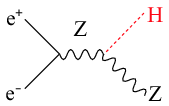
\includegraphics[width = 0.9\textwidth]{Pictures/Higgs/Chapter_Theory_figs_ZHdiagram.png}
            \caption{Higgs-Strahlung}
            \label{fig:higgsStrahlung}
        \end{subfigure}
        ~%\qquad
         %add desired spacing between images, e. g. ~, \quad, \qquad, \hfill etc. 
          %(or a blank line to force the subfigure onto a new line)
        \begin{subfigure}[t]{0.3\textwidth}
            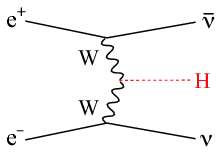
\includegraphics[width = 0.9\textwidth]{Pictures/Higgs/Chapter_Theory_figs_nunuHdiagram.png}
            \caption{$WW$-fusion}
            \label{fig:WW-fusion}
        \end{subfigure}
        ~%\qquad
         %add desired spacing between images, e. g. ~, \quad, \qquad, \hfill etc. 
          %(or a blank line to force the subfigure onto a new line)
        \begin{subfigure}[t]{0.3\textwidth}
            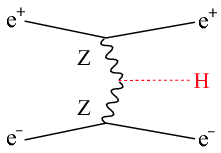
\includegraphics[width = 0.9\textwidth]{Pictures/Higgs/HiggsProd_eeH.png}
            \caption{$ZZ$-fusion}
            \label{fig:ZZ-fusion}
        \end{subfigure}
        \caption{Feynman diagrams of the main Higgs production at the ILC \cite{Asner2013}\cite{tian}.}
        \label{fig:higgsProduction}
    \end{figure}    
    
    $WW$-fusion occurs only with left-handed electrons associated with right-handed positrons.
    Thus, by modifying the beam's polarisation, the signal mixture can be changed, as well as the background processes.

    \begin{figure}[!h]
      \centering
      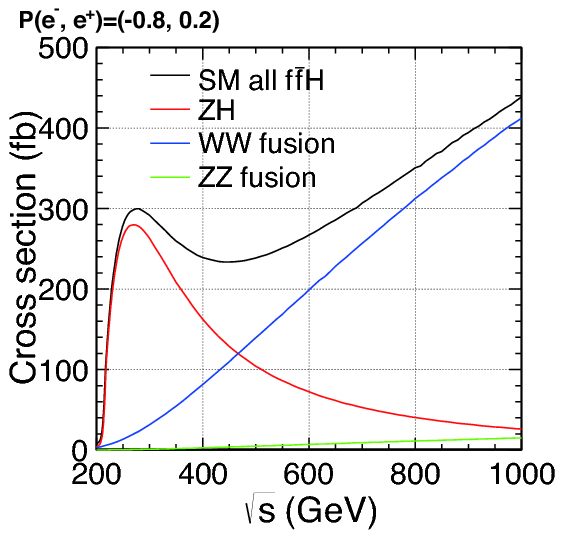
\includegraphics[width = 0.65\textwidth]{Pictures/Higgs/higgs_xsec_P-8_3.png}
      \caption{The cross section production of the Higgs boson with a mass of 125 GeV \cite{Asner2013}.}
      \label{fig:higgsXsec}
    \end{figure}

    \begin{figure}[!h]
      \centering
      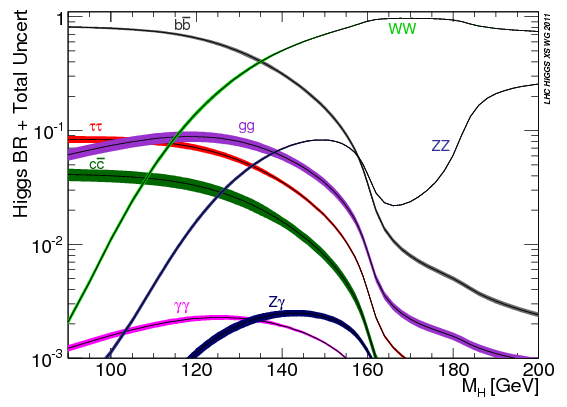
\includegraphics[width = 0.7\textwidth]{Pictures/Higgs/BRTotalUncertBands_lm.png}
      \caption{The Higgs boson branching ratio with the branching ratio uncertainties for the Higgs boson mass varying from $80$ to $200~\rm{GeV}$ \cite{Denner:2011mq}.}
      \label{fig:higgsProd}
    \end{figure}

    \subsection{Higgs boson studies}
    
    Determining the main characteristics of the Higgs boson will help to understand the mass generation mechanism.
    In the following section, the different studies performed at the \gls{LHC}, as well as the one that will be done at the \gls{ILC}, are presented.

    The \gls{ILC} will do all measurements already done by the \gls{LHC} (mass, spin, branching ratio) but the \gls{ILC} will perform model independent measurement.

    \subsubsection{Mass measurement}
    \label{sec:massRecoil}

    The mass of the Higgs boson measured at the \gls{LHC} is $M_{H} = 125.7 \pm 0.4 ~\rm{GeV}$ \cite{Agashe:2014kda}.
    In the case of the \gls{ILC}, this measurement will be performed at the peak production of Higgs-strahlung.
    The well defined four-momentum initial state allows the measurement of the Higgs boson mass regardless its decay products.
    The Higgs boson invariant mass $m_H$ can be calculated by using the recoil technique:

    \begin{equation}
      M^2_H = s + M^2_Z - 2 \sqrt{s}\left(E_{1} + E_{2}\right),
    \end{equation}
    where $M_Z$ is the mass of the $Z$ boson, $E_1$ and $E_2$ are the energies of the $Z$ decay products. 
    This technique works well for the $Z$ boson decaying into leptons at the centre-of-mass energy $\sqrt{s} = 250~\rm{GeV}$.
    However, this method can not be performed for a Higgs boson decaying into quarks at the same energy. 
    The $Z$ and the Higgs bosons are produced almost at rest, thus, the identification of the jets coming from the $Z$ boson to the ones coming from the Higgs boson is more difficult.
    Nevertheless, at higher energy ($\sqrt{s} = 500~\rm{GeV}$), the two bosons are boosted enough to separate their jets and then to reapply the recoil mass.
    Depending on the decay channel of the $Z$ boson, the statistical precision on the mass measurement varies between $40~\rm{MeV}$ (for $Z \rightarrow \mu^+\mu^-$) to $80~\rm{MeV}$ (for $Z \rightarrow e^+e^-$) and can reach $32~\rm{MeV}$ by combining the two results.
    
    \subsubsection{Spin measurement}

    Besides the mass measurement of the Higgs boson, which will be done at the centre-of-mass energy $\sqrt{s} = 250~\rm{GeV}$, studies will be performed to determine its spin and its CP-violation.
    The cross-section of the Higgs-strahlung process depends on the spin and the CP-violation of the Higgs boson.
    If the cross-section follows $s$, then the Higgs boson has a spin-0 and is CP-even, whereas a $\sqrt{s}^3$ dependency indicates a CP-odd Higgs boson.
    From the \gls{LHC} analysis, it has been determined that a spin-1 Higgs boson is forbidden because of the di-photon channel observation \cite{TheATLASCollaboration2013}.

    \subsubsection{Branching ratio measurement}

    Different decay channels were studied at the \gls{LHC}.
    The branching ratio of the Higgs boson to bosons were measured ($WW$, $ZZ$, $\gamma \gamma$, $gg$), as well as the branching ratio of the Higgs boson to second and third generations of fermions ($b\overline{b}$, $t\overline{t}$, $\mu \mu$ and $\tau \tau$).
    The properties of the \gls{ILC} beam allow the measurements of the Higgs boson couplings to the particles defined in the \gls{SM}.
    Thus, the following decay modes are accessible: $b\overline{b}$, $WW$, $ZZ$, $gg$, $c\overline{c}$, $\tau \tau$, $\gamma \gamma$, $\gamma Z$.
    One particularly interesting channel is $H \rightarrow c\overline{c}$, which will constraint the parameters to build detectors, specifically the vertex detector. 
    This measurement is also interesting because $c$-quark is an up-type quark that can be seen distinctly from down-type quarks.
    Nowadays, this measurement at the \gls{LHC} is challenging because of the \gls{QCD} background.
    Moreover, it is difficult to distinguish the vertices emerging from $b$-quarks to the one coming from $c$-quarks.
    Figure~\ref{fig:coupling} depicts the mass-coupling relation of the Higgs boson to the particles of the \gls{SM}.
    Any deviations from the Higgs boson fermionic coupling would indicate multiple Higgs boson states.

    \begin{figure}[!h]
      \centering
      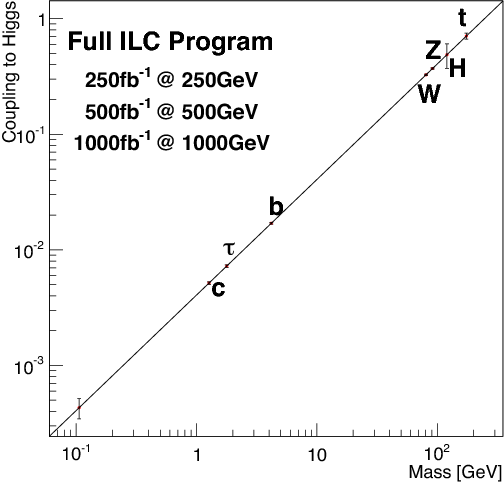
\includegraphics[width = 0.5\textwidth]{Pictures/Higgs/Chapter_Theory_figs_mass-coupling1TeV.png}
      \caption{Mass-coupling relation of the Higgs boson to the particles defined in the standard model \cite{tian}.}
      \label{fig:coupling}
    \end{figure}

  \section{Analysis of simulated data}
  
    The following section is dedicated to the analysis of simulated data of the \gls{ILC}.
    The goal of the analysis is to perform a study of the Higgs boson production at the center-of-mass energy $\sqrt{s} = 350~\rm{GeV}$ for a luminosity of $250~\rm{fb}^{-1}$.
    Nevertheless, due to the restricted time to conduct this thesis, this section introduces the tools and some results of the analysis.

  \subsection{Simulation set-up}  
  \label{subsec:ILCSOFT}

    The physics events are generated with Monte-Carlo simulation tools and are performed with different software.
    The collisions of electrons and positrons is done with the software WHIZARD \cite{WHIZARD}.
    It supports the \gls{SM} processes, as well as a large variety of BSM models.
    For linear collider physics, the beamstrahlung, the \gls{ISR} and the beam polarisation are simulated, but the hadronisation and fragmentation are not implemented and the simulation of those events was performed with PYTHIA \cite{PYTHIA}.
  
    The linear collider community has developed Monte-Carlo simulation and analysis software frameworks dedicated to a future linear collider, such as the \gls{ILC}. 
    The different packages developed by the community are grouped into the ILCSoft framework \cite{ilcsoft}.
    %The ILCSoft provides a large variety of software packages which were developed for the linear collider community\cite{ilcsoft}.
    It includes software for Monte-Carlo simulation, as well as software for test beam analysis (see chapter~\ref{chap:X0}) and other tools.
    The main package is the \gls{LCIO}, a persistence framework and event data model for linear collider detector studies \cite{lcio}. 
    It provides a common data format and event data model for both the simulation studies and the analysis framework in order to share results and compare reconstruction algorithms.

    Afterward the physics events are generated, the particle interaction inside the detector is simulated with Mokka \cite{Mokka}.
    The software is based on GEANT4 simulation toolkit \cite{GEANT4} and is part of ILCSoft.
    For the analysis, the detector model used is ILD\_o1\_v05.
    This model simulates the dead areas due to cabling, cooling system and mechanical structure and has a silicon-tungsten electromagnetic calorimeter, as well as an analog hadronic calorimeter.
    
    The detector geometry is described by an XML steering file and is used as an interface during the data reconstruction and analysis.
    This is managed by the \gls{GEAR} software \cite{GEAR}.

    Finally, the events are reconstructed with the \gls{Marlin} package \cite{MARLIN}.
    It is a C++ software framework used for the data reconstruction and data analysis and it handles \gls{LCIO} data format.
    The different steps of the analysis or the reconstruction are grouped into modules, also called processors that read an input file, perform the defined tasks and write an output file that could be processes by another \gls{Marlin} module.
    A steering file written in XML is used to select the processors to use and the order of their execution time.

  \subsection{Event generation}
     
     \subsubsection{Event samples}

     The \gls{ILD} generator group has produced signal and background samples for two different polarisations:  $\mathcal{P}_{e^-,e^+} = (-1,+1)$ and $\mathcal{P}_{e^-,e^+} = (+1,-1)$.
     Although the planned polarisation are $\mathcal{P}_{e^-,e^+} = (-0.8,+0.3)$ and  $\mathcal{P}_{e^-,e^+} = (+0.8,-0.3)$, the simulated beam polarisation is re-weighted according to:
     
     \begin{equation}
       \begin{array}{lrc}
       \sigma_{\mathcal{P}_{e^-,e^+}} & = & \frac{(1 - P_{e^-})(1+P_{e^+})}{2} \sigma_{LR} + \frac{(1+P_{e^-})(1-P_{e^+})}{2} \sigma_{RL}, \\
       \sigma_{-0.8,+0.3} & = & 0.585 \times \sigma_{LR} + 0.035 \times \sigma_{RL}, \\
       \sigma_{+0.8,-0.3} & = & 0.035 \times \sigma_{LR} + 0.585 \times \sigma_{RL}.
       \end{array}
     \end{equation}

     The cross-section $\sigma_{LR}$ is for the polarisation $\mathcal{P}_{e^-,e^+} = (-1,+1)$, whereas $\sigma_{RL}$ is the cross-section of the polarisation $\mathcal{P}_{e^-,e^+} = (+1,-1)$.
     On the one hand, the Higgs-strahlung and the $WW$-fusion processes are equally important for the beam polarisation  $\mathcal{P}_{e^-,e^+} = (-0.8,+0.3)$, leading to a larger $\nu\overline{\nu} H$ cross-section.
     On the other hand, the polarisation $\mathcal{P}_{e^-,e^+} = (-0.8,+0.3)$ is used to perform a cross-check measurement.
     The $W$-boson cannot couple to right-handed electrons and left-handed positrons.
     Thus, the $WW$-fusion process is largely suppressed.
     Besides, the $Z$-boson depends on the isospin and the Higgs-strahlung contribution is also reduced but not suppressed.
     The same effect occurs on the backgrounds leading to a smaller background contamination of the signal and a cleaner signal sample for Higgs-strahlung.

     The data set is scaled to an integrated luminosity of $250~\rm{fb}^{-1}$ for each beam polarisation.

  \subsubsection{Signal}

    The signal to study is the final state $\nu\overline{\nu}H$, on which the Higgs boson decays into a pair of quarks, such as $H \rightarrow b\overline{b}$ and $H \rightarrow c\overline{c}$, or a pair of gluons $H \rightarrow gg$. 
    The other decay modes are considered here as a source of background. 
    The dominant production processes leading to this final state are Higgs-strahlung and $WW$-fusion.
    Their leading order Feynman diagrams are displayed respectively on figure~\ref{fig:higgsStrahlung} and~\ref{fig:WW-fusion}.
    Although the neutrinos produced in the $WW$-fusion process are only $\nu_{\rm{e}}$ and all neutrino flavors are equi-probable in Higgs-strahlung, the neutrino flavors cannot be detected and only the missing energy is the signature of neutrino production.

    \begin{figure}[!h]
      \centering
      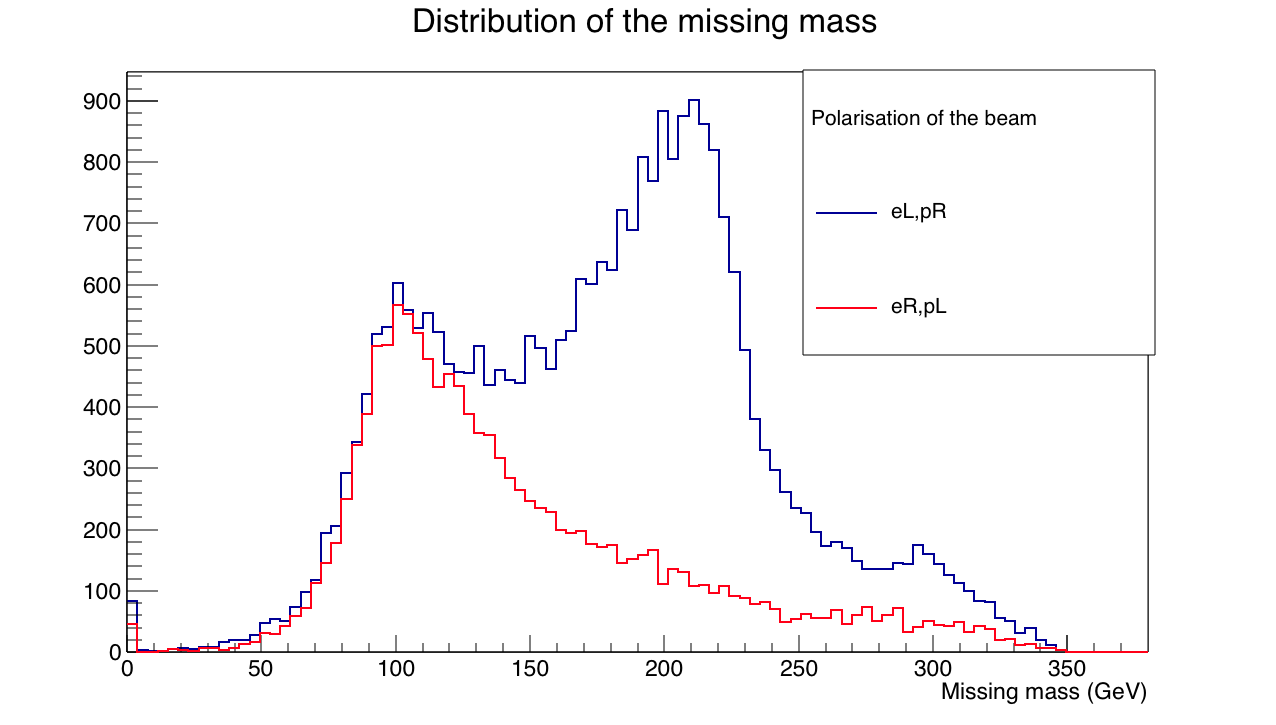
\includegraphics[width = 0.9\textwidth]{Pictures/Higgs/mMiss.png}
      \caption{Distribution of the missing mass with different beam polarisations and for the Higgs-strahlung and $WW$-fusion leading to $\nu\overline{\nu}H$ final state.
      The background contribution is not taken into account here.}
      \label{fig:mMiss}
    \end{figure}

    Figure~\ref{fig:mMiss} represents the distribution of the missing mass for the signal events for the two polarisations considered at the \gls{ILC}.
    The first effect of the polarisation is the suppression of $WW$-fusion contribution and also a reduction of Higgs-strahlung for right-handed electrons and left-handed positrons.
    For the other polarisation, the missing mass distribution shows three peaks. 
    Once centered around $90~\rm{GeV}$ corresponding to the decay of the Z-boson into a pair of neutrinos.
    The second peak is broader and its maximum is at $200~\rm{GeV}$.
    This comes from $WW$-fusion.
    A third peak is visible at $300~\rm{GeV}$ and is coming from the Higgs boson decaying leptonically and is considered as a source of background.    

  \subsubsection{Background processes}

    The signal hypothesis is that the final state consists of two jets coming from the hadronic decay of the Higgs boson, as well as missing energy coming from the undetected neutrinos produced by the $Z$ boson decay.
    Nonetheless, this signal is drowned out by the background processes.
    The background consists of events with the same final states as the signal, called irreducible background and the events with a similar detector response.
    Their contributions depend on the beam polarisation.
    For example, the cross-section for a beam polarisation $\mathcal{P}_{e^-,e^+} = (+0.8,-0.3)$ is smaller by an order of magnitude due to the $W$ boson.

    Two irreducible backgrounds are considered here, the one involving a $W$-boson exchange and the one with a $Z$-boson exchange.
    The final state of backgrounds contains two jets with missing energy.
    The cross-section of this processes is few times larger than the signal one.
    Nevertheless, the final state with quarks is more likely than the final state with two gluons due to the loop formed in the final state on which the gluons are emitted.

    The background involving $W$-bosons, such as $e^{-}e^{+} \rightarrow W^{\pm}e^{\pm}\nu_{e} \rightarrow e^{\pm}\nu_{e}q\overline{q}$ is two orders magnitude bigger than the signal cross-section.
    The neutrino produced carries a large transverse momentum, whereas the electron or positron has a low transverse momentum.
    Hence, it can be undetected and be considered as missing energy.
    
    The $W$-pair production can lead to semi-leptonic, hadronic and leptonic decay modes.
    The semi-leptonic mode consists of two jets and a lepton with its associated neutrino ($e^{+}e^{-} \rightarrow W^+W^- \rightarrow \nu_{l}l^{\pm}q\overline{q}$) and it is the major background process for the $W$-pair production.
    This background is detected by looking for an isolated lepton.
    Nevertheless, the lepton could escape the detector undetected or be inside a jet.
    The second $W$-pair production is the hadronic decay on which there is no missing energy ($e^{+}e^{-} \rightarrow W^+W^- \rightarrow q\overline{q} q\overline{q}$).
    This background is reduced by applying cuts on the missing momentum and the di-jet invariant mass.
    The last contribution is the leptonic final state, which is easy to distinguish from the signal.
    Thus, it is not considered in the study. 

    The $Z$-pair background is ten times smaller than the $W$-pair production.
    The  $e^+e^- \rightarrow ZZ \rightarrow \nu_{l}\overline{\nu_{l}}q \overline{q}$ process is an irreducible background.
    The hadronic decay $e^+e^- \rightarrow ZZ \rightarrow q\overline{q} q\overline{q}$ is reduced by cutting on the missing momentum and the di-jet invariant mass.
    The semi-leptonic process $e^+e^- \rightarrow ZZ \rightarrow l^+l^- q\overline{q}$ is easier to detect because of the second isolated lepton in the event.

    Finally, the last background to take into account is the one with the Higgs boson produced in the final state.
    Higgs-strahlung can lead to $q\overline{q}H$ and $l^{\pm}l^{\mp}H$ and has a cross-section three times larger than the signal, but it is easily identified due to the absence of the neutrino.
    All the decay mode of the Higgs boson different from $H \rightarrow b\overline{b}$, $H \rightarrow c\overline{c}$ and $H \rightarrow gg$ are considered as part of the background.

    \begin{figure}[!h]
      \centering
      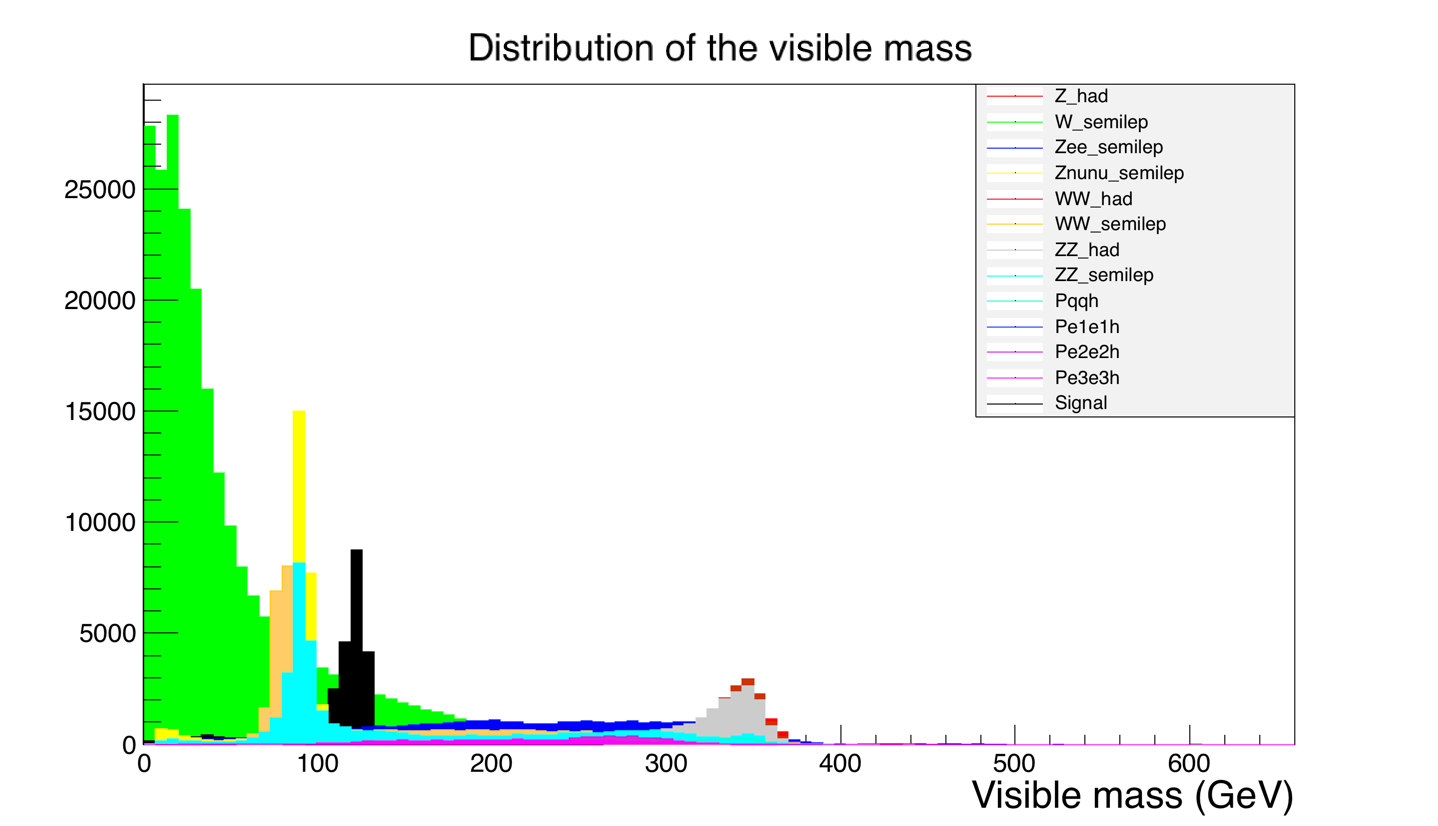
\includegraphics[width = 0.9\textwidth]{Pictures/Higgs/mVis_all.png}
      \caption{Distribution of the visible mass for the signal and background together and the polarisation $\mathcal{P}_{e^-,e^+} = (-0.8,+0.3)$.}
      \label{fig:mVisAll}
    \end{figure}

    Figure~\ref{fig:mVisAll} shows the distribution of the visible mass for all the processes taken into account during the analysis and a beam polarisation $\mathcal{P}_{e^-,e^+} = (-0.8,+0.3)$.
    A selection has to be performed in order to isolate the peak at $125~\rm{GeV}$.

  \section{Results}
 
    \subsection{Event reconstruction}

    The assumption to study the $H \nu\nu$ channel is to reconstruct a final state which is giving two jets and missing energy in the detector response.
    %The reconstruction consists to select and highlight this detector response.

    The first step consists of identifying the events containing of isolated leptons in the final state and to remove them from the event sample.
    The leptons detected outside a jet are considered as a source of background.
    Thus, a neural network is used to identify the different leptons in an event and to check if they belong to a jet.
    This selection is based on different criteria, like the vertex information, the energy deposited inside the \gls{ECAL}, the \gls{HCAL} and the muon system. 
    The processor used for the identification is called \textit{IsolatedLeptonTagger} and has a veto efficiency of roughly $90~\%$.
    The $10~\%$ of leptons undetected are coming from events in which the leptons are moving into the forward region and they could escape the detector without being identified by the processor.
    A better selection is done after the jet reconstruction and is discussed later.

    A second source of background is coming from the $\gamma \gamma$ overlay interactions which produce low $p_{t}$ hadrons.
    These hadrons with a small transverse momenta and a small relative angle to the beam axis are detected as jet-like objects in the forward region of the detector.
    The identification of the beam jets is based on the $k_{T}$ algorithm \cite{Cacciari2008}.
    It consists in defining a "distance" $d_{ij}$ between two particles and to find the first closest constituent.
    
    \begin{equation}
      \begin{array}{lcl}
        d_{ij} & = & \frac{\rm{min}\left(p^2_{T_i}, p^2_{T_j}\right) \cdot \Delta R^2_{ij}}{R^2}, \\
        d_{i}  & = & p^2_{T_i},
      \end{array}
    \end{equation}
    with $\Delta R^2_{ij} = \left( y_{i} - y_{j}\right)^2 + \left( \phi_{i} - \phi_{j}\right)^2$, $y_{i}$ the pseudo rapidity, $\phi_{i}$ the azimuthal angle and $p_{T_i}$ the transverse momentum of the particle studied.
    The minimum between $d_{ij}$ and $d_{i}$ is calculated.
    If $d_{ij}$ is the minimum value, then, the particles $i$ and $j$ are merged into a jet candidate, they are then removed from the physics list and the jet candidate is added instead.
    If the minimum value is $d_{i}$, the particle is considered to be part of the beam jet and is removed from the particle lists.
    This algorithm is repeated iteratively until the number of jets created is equal to the number of jets expected.
   
    After removing the isolated leptons and the low $p_{t}$ hadrons from the physics list, the jet clustering and the flavor tagging processors are applied. 
    Due to the $k_{T}$ algorithm, which removes particle from the physics list, the vertex finder is run again before using the jet clustering algorithm.

  \subsection{Event selection}

  To improve the signal to noise ratio, an event selection is performed by applying different cuts that reduce the background contribution.
  The order and the performances of the selection cuts are determined by maximising the significance $s$, which is:

  \begin{equation}
    s = \frac{\rm{N_{sig}}}{\sqrt{\rm{N_{sig}}+ \rm{N_{bg}}}},
  \end{equation}
  with, $\rm{N_{bg}}$ the number of remaining background and $\rm{N_{sig}}$, the number of remaining signal.
  The maximisation of $s$ is needed to minimise the statistical error.
  Firstly, the procedure starts with the definition of a collection of observables that could help to discriminate the signal from the background.
  Then, a test of the possible cut values is performed in a given range and for a given step size.
  The value leading to the largest significance is chosen as the optimum observable and is the first selection variable which is applied to a signal sample (containing $WW$-fusion and Higgs-strahlung processes) and the least tight constraint is selected in order to maintain a good signal efficiency.
  Finally, the cut values of this optimum observable is applied on the complete data set and the procedure is applied again.

  The first observable to be applied is the veto information used to find any isolated lepton.
  As already mentioned, the \textit{IsolatedLeptonTagger} processor has a veto efficiency of roughly $90~\%$. 

  The second observable is the visible transverse momentum $P_{\rm{t,vis}}$ of the di-jets. 
  \begin{equation}
    \begin{array}{lcl}
      P_{\rm{t,vis}} = \sqrt{P^2_{x,vis} + P^2_{y,vis}}, \\
      P_{\rm{x/y,vis}} = P_{\rm{x/y,j1}} + P_{\rm{x/y,j2}}. 
    \end{array}
  \end{equation}
 
  $ P_{\rm{x/y,j1}}$ and $ P_{\rm{x/y,j2}}$ are the visible momentum in the $x$ and $y$-directions for the two jets $j1$ and $j2$.

  The third observable is the invariant visible mass $m_{\rm{vis}}$, which is the signal signature.

  \begin{equation}
   \rm{m_{vis}} = \sqrt{E^2_{\rm{vis}} - \overrightarrow{P}^{\,2}_{\rm{vis}}},
  \end{equation}
  with $E_{\rm{vis}}$ and $P_{\rm{vis}}$ the visible energy and momentum of the event.
  The expected visible mass is $\rm{m_H} = 125~\rm{GeV}$ and its width is mainly driven by the jet energy resolution.

%    \begin{sidewaystable}
%    \scriptsize{
%    \flushleft
%      \begin{tabular}{c c c c c c c}
%           \hline
%           {Process} & {Cross Section (fb)} & {Events number} & \text{No isolated leptons} & {$35 <~\rm{{P}_{t}^{vis}} < 155~\rm{GeV} $} & {$95 <~\rm{m_{vis}}< 140~\rm{GeV}$} & {$-1 <~\rm{\cos{\alpha}}< 0.22$} \tabularnewline \hline
%           \hline
%           Zhad            &$ 3.86\times 10^{4} $&$	1.27\times 10^{7} $&$ 1.26\times 10^{7} $&$ 1.09\times 10^{5} $&$ 5.79\times 10^{2} $ &$	5.05\times 10^{2}  $\tabularnewline 
%           WW had          &$ 6.53\times 10^{3} $&$	2.16\times 10^{6} $&$	2.14\times 10^{6} $&$	5.27\times 10^{3} $&$	6.29              $ &$	6.29               $\tabularnewline 
%           WW semilep      &$ 8.16\times 10^{3} $&$	2.69\times 10^{6} $&$	1.17\times 10^{6} $&$	6.38\times 10^{5} $&$	1.13\times 10^{5} $ &$  6.26\times 10^{4}  $\tabularnewline 
%           ZZ had          &$ 6.01\times 10^{2} $&$	1.98\times 10^{5} $&$	1.97\times 10^{5} $&$	2.74\times 10^{3} $&$	1.20              $ &$  6.20\times 10^{-1} $\tabularnewline 
%           ZZ semilep      &$ 5.65\times 10^{2} $&$ 1.86\times 10^{5} $&$ 1.40\times 10^{5} $&$ 7.49\times 10^{4} $&$ 1.46\times 10^{4} $ &$  8.20\times 10^{3}  $\tabularnewline 
%           singleW semilep &$ 1.63\times 10^{3} $&$ 5.36\times 10^{5} $&$	2.24\times 10^{4} $&$	8.79\times 10^{3} $&$	1.65\times 10^{3} $ &$	1.63\times 10^{3}  $\tabularnewline 
%           singleZee semi  &$ 3.10\times 10^{2} $&$	1.02\times 10^{5} $&$	1.30\times 10^{4} $&$	2.17\times 10^{1} $&$	7.00\times 10^{-2}$ &$	7.00\times 10^{-2} $\tabularnewline 
%           singleZnn semi  &$ 3.55\times 10^{2} $&$	1.17\times 10^{5} $&$ 1.17\times 10^{5} $&$	8.38\times 10^{4} $&$	1.62\times 10^{4} $ &$	1.19\times 10^{4}  $\tabularnewline 
%           Higgs BG        &$ 1.62\times 10^{2} $&$	5.34\times 10^{4} $&$ 4.19\times 10^{4} $&$ 4.59\times 10^{3} $&$	1.93\times 10^{2} $ &$	1.43\times 10^{2}  $\tabularnewline 
%           HiggsToOther    &$ 3.05\times 10^{1} $&$	1.01\times 10^{4} $&$	6.66\times 10^{3} $&$	4.95\times 10^{3} $&$ 3.45\times 10^{3} $ &$	2.64\times 10^{3}  $\tabularnewline 
%           \hline						
%           Background     &$ 5.69\times 10^{4} $&$  1.88\times 10^{7} $&$	1.65\times 10^{7} $&$	9.31\times 10^{5} $&$ 1.50\times 10^{5} $ &$  8.76\times 10^{4}  $\tabularnewline 
%           Signal	        &$ 6.82\times 10^{2} $&$  2.25\times 10^{4} $&$	2.23\times 10^{4} $&$	1.82\times 10^{4} $&$	1.66\times 10^{4} $ &$	1.57\times 10^{4}  $\tabularnewline 
%           Significance   &                     &$	5.19              $&$	5.48 $             &$	1.87\times 10^{1} $&$	4.06\times 10^{1} $ &$  4.88\times 10^{1}  $\tabularnewline 
%     \end{tabular}
%    }
%    \caption{Cut flow chart with three first cuts applied.}
%    \label{tab:cutFlow}
%  \end{sidewaystable}

  \begin{table}
    \begin{tabular}{c c c c}
      \hline
      Process                                     & Background          & Signal              & Significance  \tabularnewline
      \hline
      \hline
      Cross-section (fb)                          & $5.69 \cdot 10^{4}$ & $6.82 \cdot 10^{2}$ &               \tabularnewline
      \hline
      Expected event number                       & $1.88 \cdot 10^{7}$ & $2.25 \cdot 10^{4}$ & $5.2$         \tabularnewline
      No isolated leptons                         & $1.65 \cdot 10^{7}$ & $2.23 \cdot 10^{4}$ & $5.5$         \tabularnewline
      {$35 <~\rm{{P}_{t}^{vis}} < 155~\rm{GeV} $} & $9.31 \cdot 10^{5}$ & $1.82 \cdot 10^{4}$ & $18.7$        \tabularnewline
      {$95 <~\rm{m_{vis}}< 140~\rm{GeV}$}         & $1.50 \cdot 10^{5}$ & $1.66 \cdot 10^{4}$ & $40.6$        \tabularnewline
      {$-1 <~\rm{\cos{\alpha}}< 0.22$}            & $8.76 \cdot 10^{4}$ & $1.57 \cdot 10^{4}$ & $48.8$        \tabularnewline
      $26 < (\rm{N.R.C > 1GeV}) < 99$             & $2.25 \cdot 10^{4}$ & $1.19 \cdot 10^{4}$ & $56.3$        \tabularnewline
      $0.11 < \rm{DurhamjD2ym} < 1$               & $1.78 \cdot 10^{4}$ & $1.05 \cdot 10^{4}$ & $62.3$        \tabularnewline
      $0 < \rm{abs(RefinedjPzvis)} < 113~\rm{GeV}$& $1.51 \cdot 10^{4}$ & $1.01 \cdot 10^{4}$ & $63.5$        \tabularnewline
      $156 < \rm{RefinedjEmiss} < 230~\rm{GeV}$   & $1.37 \cdot 10^{4}$ & $9.85 \cdot 10^{3}$ & $64.1$        \tabularnewline      
      \hline %----------------------------
    \end{tabular}
    \caption{Cut-flow table for a beam polarisation $\mathcal{P}_{e^{-},e^{+}} = (-0.8, +0.3)$.}
    \label{tab:cutFlow}
  \end{table}

  Table~\ref{tab:cutFlow} summarises the order of the different cut selection for different observables applied on the simulated data set.
  After eight consecutives cuts, the background contribution is three orders smaller, whereas the signal is almost one order smaller than the beginning.
  Nevertheless, the significance is still less than 70 and applying more cuts strongly affects the signal.

  \section{Outlook}

  To preserve the sample quality, it is rather better to use a \gls{MVA} method to extract the signal from the background.
  The complete information is then used simultaneously to find the best sets of variables.
  This analysis was already performed and a \gls{MVA} method was used, achieving a significance above $70$.

  The next step of this analysis is to focus on the decay mode of the Higgs boson into two pairs of charmed quarks and to optimise the flavor tagging performances to separate more accurately the $b$ and $c$ quarks events.
  For the events and the detector simulated in this chapter, the vertex detector geometry was not optimised and was made of five single sided layers.
  Nevertheless, the double sided option has to be investigated.
  This geometry offers multiple possibilities, like using two different types of sensors on the same ladder or the possibility of two point measurements per ladder for a track.
  One side could be equipped with ultra-fast integration time ($\mathcal{O} \sim 1~\rm{\mu s}$) sensors, whereas the other side could embed sensors with an excellent pointing resolution ($\sigma_{\rm{s.p}} \leq 3~\rm{\mu m}$).
  With two sensors on the same mechanical structure, a track is reconstructed by two points of measurement.
  Thus, these two measurements could be combined together to form "mini-vectors".
  Studying the "mini-vectors" could help to identify the beamstrahlung from the collision events.



  %This is important to determine the geometry configuration and the technology used to build the vertex detector.
  %The study could consist first to compare the branching ratio measured with two different detector geometries. 
  %The one used in this analysis was made of a five single sided layers, but to decide which structure, like single or double-sided ladder, the analysis as to be ran again.
  %One possible vertex detector considered is made of three double-sided layers.
  %On one side of a ladder, sensors with an ultra-fast integration time ($\mathcal{O} \sim 1~\rm{\mu s}$) and on the other side, sensors with an excellent pointing resolution ($\sigma_{\rm{s.p}} \leq 3~\rm{\mu m}$).

